Relacionado a los resultados del algoritmo 1. Este algoritmo tomó un total de 17 generaciones. Se obtuvo un aptitud promedio final de 36,557.61 km y su mejor individuo consiguió una aptitud de 36,557.61 km. El proceso de convergencia se puede observar en la Figura \ref{fig:AG_1}.

\begin{figure}[htbp]
	\centering
	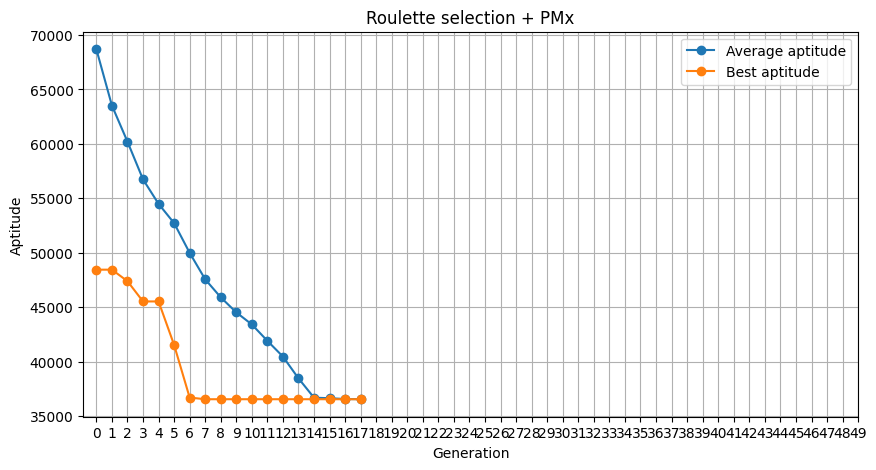
\includegraphics[width=0.6\textwidth]{roulette_selection_pmx}
	\caption{Evolución de la aptitud de los individuos del algoritmo 1.}
	\label{fig:AG_1}
\end{figure}

Relacionado a los resultados del algoritmo 2. Este algoritmo tomó un total de 50 generaciones. Se obtuvo un aptitud promedio final de 31,214.21 km y su mejor individuo consiguió una aptitud de 29,746.86 km. El proceso de convergencia se puede observar en la Figura \ref{fig:AG_2}.

\begin{figure}[htbp]
	\centering
	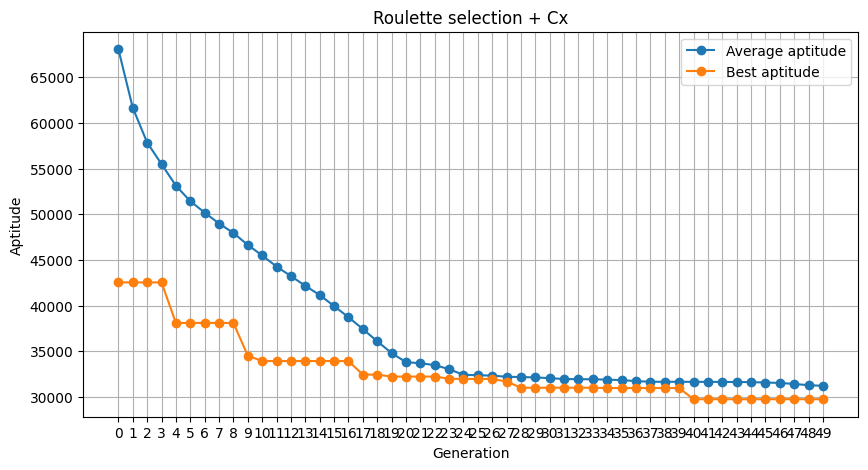
\includegraphics[width=0.6\textwidth]{roulette_selection_cx}
	\caption{Evolución de la aptitud de los individuos del algoritmo 2.}
	\label{fig:AG_2}
\end{figure}

\newpage
Relacionado a los resultados del algoritmo 3. Este algoritmo tomó un total de 17 generaciones. Se obtuvo un aptitud promedio final de 32,423.60 km y su mejor individuo consiguió una aptitud de 30,304.17 km. El proceso de convergencia se puede observar en la Figura \ref{fig:AG_3}.

\begin{figure}[htbp]
	\centering
	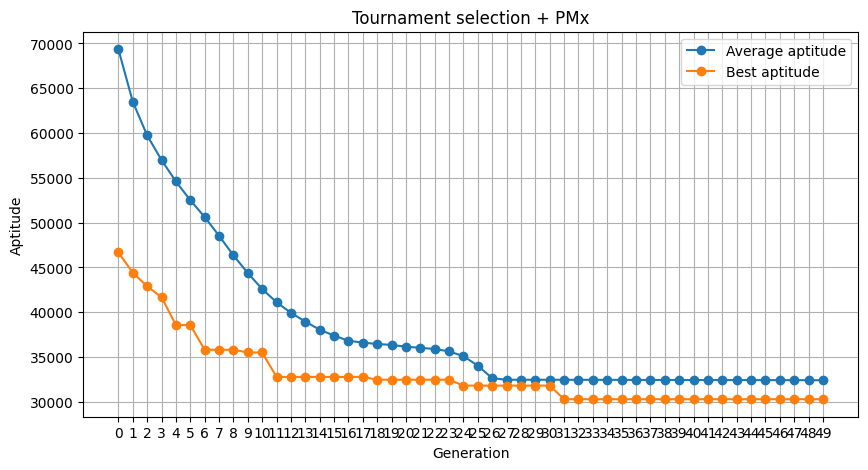
\includegraphics[width=0.6\textwidth]{tournament_selection_pmx}
	\caption{Evolución de la aptitud de los individuos del algoritmo 3.}
	\label{fig:AG_3}
\end{figure}

Relacionado a los resultados del algoritmo 4. Este algoritmo tomó un total de 17 generaciones. Se obtuvo un aptitud promedio final de 25,060.90 km y su mejor individuo consiguió una aptitud de 24,571.73 km. El proceso de convergencia se puede observar en la Figura \ref{fig:AG_4}.

\begin{figure}[htbp]
	\centering
	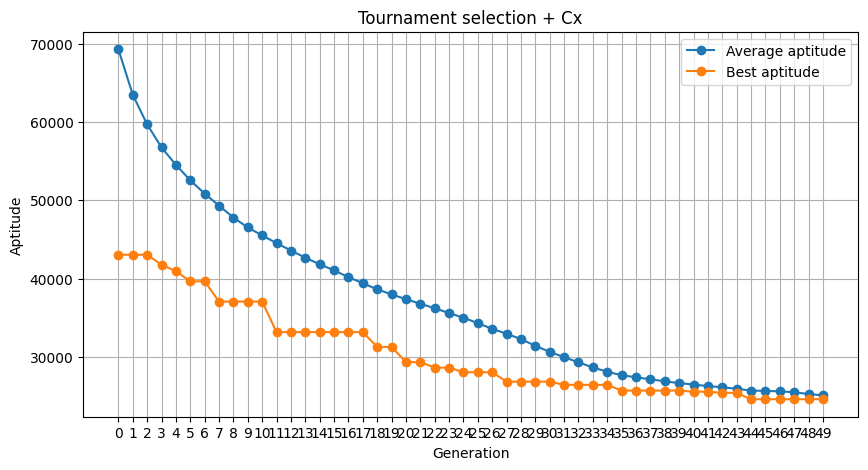
\includegraphics[width=0.6\textwidth]{tournament_selection_cx}
	\caption{Evolución de la aptitud de los individuos del algoritmo 4.}
	\label{fig:AG_4}
\end{figure}

Todos estos resultados se puden resumir en la Tabla \ref{tab:RES}, en la cual se puede observar que los mejores resultados fueron los obtenidos por el algoritmo 4.

\begin{table}[htbp]
\centering
\caption{Resumen de resultados de todos los algoritmos.}
\begin{tabular}{lccc}
\hline
\hline
Algoritmo & Mejor Aptitud {[}km{]} & Aptitud Promedio {[}km{]} & Total de individuos \\\hline
Algoritmo 1 & 36,557.61 & 36,557.61 & 100 \\
Algoritmo 2 & 29,746.86 & 31,214.21 & 250 \\
Algoritmo 3 & 30,304.17 & 32,423.60 & 500 \\
Algoritmo 4 & 24,571.73 & 25,060.90 & 1,000 \\\hline
\end{tabular}
\label{tab:RES}
\end{table}